\documentclass[10pt,aspectratio=149]{beamer}

% All the boilerplate is in raslides.sty
% Note that this also pulls in a custom vogtwidebar.sty
\usepackage{raslides}

\author{Ji\v{r}\'i Lebl}

\institute[OSU]{%
Departemento pri Matematiko de Oklahoma {\^S}tata Universitato}

\title{BA: 4.2}

\date{}

\begin{document}

\begin{frame}
\titlepage
\end{frame}

\begin{frame}
\begin{definition}
Let $S \subset \R$ be a set.
A function
$f \colon S \to \R$ has a \emph{relative maximum}
at $c \in S$ if there exists a $\delta>0$
such that for all $x \in S$ where $\abs{x-c} < \delta$,
we have $f(x) \leq f(c)$.
\pause
The definition of
\emph{relative minimum}
is analogous.
\end{definition}

\pause
\begin{lemma}
Suppose $f \colon (a,b) \to \R$ is differentiable at $c \in (a,b)$,
and $f$ has
a relative minimum or a relative maximum at $c$.  Then
$f'(c) = 0$.
\end{lemma}

\pause
\textbf{Remark:}  Point $c$ where $f'(c)=0$ is called a
\emph{critical point}.

\pause
\medskip

Idea of proof:

\vspace*{-12pt}
\phantom{Idea of proof:~~~~}\scalebox{0.8}{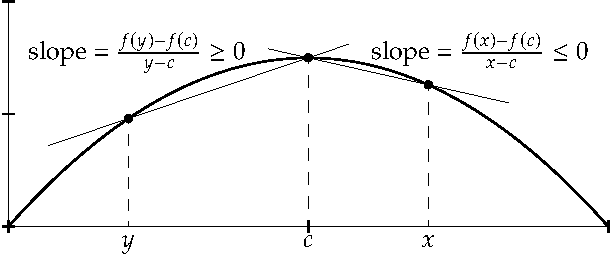
\includegraphics{../figures/critpt}}

\end{frame}

\begin{frame}

\begin{lemma}
Suppose $f \colon (a,b) \to \R$ is differentiable at $c \in (a,b)$,
and $f$ has
a relative minimum or a relative maximum at $c$.  Then
$f'(c) = 0$.
\end{lemma}

\pause
\textbf{Proof:}
Let $c$ be a relative maximum of $f$ \quad (if minimum, look at $-f$).

\pause
\medskip

$\exists$ $\delta > 0$ such that 
if $x \in (a,b)$ and $\abs{x-c} < \delta$, then ~~
$f(x)-f(c) \leq 0$.

\pause
\medskip

If $c < x < c+\delta$, then
$\displaystyle
\frac{f(x)-f(c)}{x-c} \leq 0$.

\pause
\medskip

If $c-\delta < y < c$, then
$\displaystyle
\frac{f(y)-f(c)}{y-c} \geq 0$.

\pause
\medskip

As $a < c < b$, $\exists$
$\{ x_n \}_{n=1}^\infty$ and
$\{ y_n \}_{n=1}^\infty$ in $(a,b) \cap (c-\delta,c+\delta)$,

\pause
such that $x_n > c$, $y_n < c$ for all $n \in \N$,

\pause
and
$\lim\limits_{n\to\infty} x_n = \lim\limits_{n\to\infty} y_n = c$.

%\medskip

\pause
As $f$
is differentiable at $c$,
\quad
$\displaystyle
0 \geq \lim_{n\to\infty} \frac{f(x_n)-f(c)}{x_n-c} 
\pause
=
f'(c)
\pause
=
\lim_{n\to\infty} \frac{f(y_n)-f(c)}{y_n-c}
\pause
\geq 0$.

\pause
\medskip

\thus \quad $f'(c) = 0$.
\qed

\end{frame}

\begin{frame}
\begin{theorem}[Rolle]
Let $f \colon [a,b] \to \R$ be continuous and
differentiable on $(a,b)$ such that $f(a) = f(b)$.
Then there exists a $c \in (a,b)$ such that $f'(c) = 0$.
\end{theorem}

\pause
\begin{center}
\scalebox{0.9}{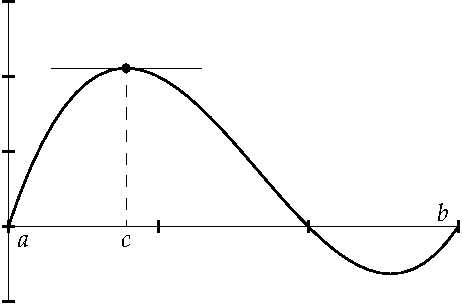
\includegraphics{../figures/rollefig}}
\end{center}

\pause
\medskip

\textbf{Example:}
It is necessary for $f'$ to exist for all $x \in (a,b)$.

\pause
Consider $f(x) \coloneqq \abs{x}$ on $[-1,1]$.
\quad
$f(-1) = f(1)$, but at no $c$ does $f'(c)=0$.
\end{frame}

\begin{frame}

\begin{theorem}[Rolle]
Let $f \colon [a,b] \to \R$ be continuous and
differentiable on $(a,b)$ such that $f(a) = f(b)$.
Then there exists a $c \in (a,b)$ such that $f'(c) = 0$.
\end{theorem}

\pause
\textbf{Proof:}
$f$ is continuous on $[a,b]$ \wthus attains an absolute min/max on $[a,b]$.

\pause
\medskip

Let $K \coloneqq f(a) = f(b)$.

\pause
\medskip

If $\exists$ $x \in (a,b)$ where $f(x) > K$,

\pause
then $\exists$ $c \in (a,b)$ where $f$ attains a maximum.

\pause
\medskip

If $\exists$ $x \in (a,b)$ where $f(x) < K$,

\pause
then $\exists$ $c \in (a,b)$ where $f$ attains a minimum.

\pause
\medskip

If $f(x) = K$ for all $x \in (a,b)$,

\pause
then $\exists$ $c \in (a,b)$ where $f$ attains a max and a min.

\pause
\medskip

In any case, the lemma applies, and $f'(c)=0$.
\qed

\end{frame}

\begin{frame}

\begin{theorem}[Mean value theorem]
Let $f \colon [a,b] \to \R$ be continuous and
differentiable on $(a,b)$.  Then there exists $c \in (a,b)$
such that \quad
$f(b)-f(a) = f'(c)(b-a)$.
\end{theorem}

\pause
\begin{center}
\scalebox{0.8}{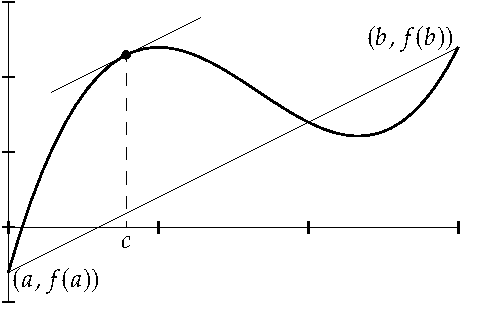
\includegraphics{../figures/mvtfig}}
\end{center}

\pause
$\frac{f(b)-f(a)}{b-a}$
is the slope of the secant line between $\bigl(a,f(a)\bigr)$ and $\bigl(b,f(b)\bigr)$.

\pause
\medskip

The slope of the secant line is the mean value of $f'$ (hence the name).

\pause
\medskip

So the average derivative is attained at $c$:
\quad
$f'(c)=\frac{f(b)-f(a)}{b-a}$.
\end{frame}

\begin{frame}
\begin{theorem}[Mean value theorem]
Let $f \colon [a,b] \to \R$ be continuous and
differentiable on $(a,b)$.  Then there exists $c \in (a,b)$
such that \quad
$f(b)-f(a) = f'(c)(b-a)$.
\end{theorem}

\pause
\textbf{Proof:}
Define 
$g \colon [a,b] \to \R$ by
\begin{equation*}
g(x) \coloneqq f(x)-f(b)-\frac{f(b)-f(a)}{b-a}(x-b) .
\end{equation*}
\pause
$g$ is differentiable on $(a,b)$,

\pause
continuous on $[a,b]$,

\pause
and $g(a) = 0$, $g(b) = 0$.

\pause
\medskip

\thus \quad (by Rolle) $\exists$
$c \in (a,b)$ such that $g'(c) = 0$.

\pause
\medskip

$0 = g'(c) = f'(c)-\frac{f(b)-f(a)}{b-a}$
\pause
\quad
\text{or}
\quad
$f(b)-f(a) = f'(c)(b-a)$.
\qed

\end{frame}

\begin{frame}
\begin{theorem}[Cauchy's mean value theorem]
Let $f \colon [a,b] \to \R$ and $\varphi \colon [a,b] \to \R$ be continuous
functions
differentiable on $(a,b)$.  Then there exists a point $c \in (a,b)$
such that
\begin{equation*}
\bigl(f(b)-f(a)\bigr)\varphi'(c) = f'(c)\bigl(\varphi(b)-\varphi(a)\bigr) .
\end{equation*}
\end{theorem}

\pause
\textbf{Proof:} Exercise.
\pause
Hint: Consider
$g(x) \coloneqq
f(x)-f(b)-\frac{f(b)-f(a)}{\varphi(b)-\varphi(a)}\bigl(\varphi(x)-\varphi(b)\bigr)$.

\end{frame}

\begin{frame}

We now solve our a differential equation:

\begin{proposition}
Let $I$ be an interval and
$f \colon I \to \R$ be differentiable such that $f'(x) = 0$
for all $x \in I$.

\pause
Then $f$ is constant.
\end{proposition}

\pause
\textbf{Proof:}
Take arbitrary $x,y \in I$ with $x < y$.

\pause
\medskip

As $I$ is an interval, $[x,y] \subset I$.

\pause
\medskip

$f|_{[x,y]}$ satisfies the mean value theorem.

\pause
\medskip

\thus \quad $\exists$ $c \in (x,y)$ such that
$\displaystyle f(y)-f(x) = f'(c)(y-x)$.

\pause
\medskip

$f'(c) = 0$
\pause
\wthus $f(y) = f(x)$
\pause
\wthus $f$ is constant.
\qed
\end{frame}

\begin{frame}
$f \colon I \to \R$ is \emph{increasing}
(resp.\  \emph{strictly increasing}) if
$x < y$ implies

$f(x) \leq f(y)$ (resp.\ $f(x) < f(y)$).

\pause
\emph{decreasing} and
\emph{strictly decreasing} is similar.

\pause
\begin{proposition}
Let $I$ be an interval and
let $f \colon I \to \R$ be a differentiable function.
%\begin{enumerate}[(i),itemsep=0.5\itemsep,parsep=0.5\parsep,topsep=0.5\topsep,partopsep=0.5\partopsep]
\begin{enumerate}[(i)]
\item
\pause
$f$ is increasing if and only if $f'(x) \geq 0$ for all $x \in I$.
\item
\pause
$f$ is decreasing if and only if $f'(x) \leq 0$ for all $x \in I$.
\end{enumerate}
\end{proposition}

\pause
\textbf{Proof:}
(i) $\Rightarrow$) Suppose $f$ is increasing.

\pause
\medskip

For all $x,c \in I$ with $x \neq c$, ~~
$\displaystyle
\frac{f(x)-f(c)}{x-c} \geq 0$.
\pause
~~
Take limit $x \to c$ to get $f'(c) \geq 0$.

\pause
\medskip

$\Leftarrow$) suppose $f'(x) \geq 0$ for all $x \in I$.

\pause
Take any $x, y \in I$ where $x < y$.  (note that $[x,y] \subset I$).

\pause
\medskip

By the mean value theorem, $\exists$ $c \in (x,y)$ s.t.
$\displaystyle
f(y)-f(x) = f'(c)(y-x)$.

\pause
\medskip

$f'(c) \geq 0$ and $y-x > 0$ \wthus $f(y) - f(x) \geq 0$ or $f(x) \leq
f(y)$
\pause
~~(so $f$ is increasing).

\pause
\medskip

(ii) is an exercise.
\qed

\end{frame}

\begin{frame}

\begin{proposition}
Let $I$ be an interval and
let $f \colon I \to \R$ be a differentiable function.
\begin{enumerate}[(i)]
\item
\pause
If $f'(x) > 0$ for all $x \in I$, then
$f$ is strictly increasing.
\item
\pause
If $f'(x) < 0$ for all $x \in I$,
then $f$ is strictly decreasing.
\end{enumerate}
\end{proposition}

\pause
\textbf{Proof:} Exercise.

\pause
\medskip

\textbf{Example:} Converse not true: 
$f(x) \coloneqq x^3$ is strictly increasing, but $f'(0) = 0$.

\end{frame}

%\begin{frame}
%
%Another application of the mean value theorem is the following result about
%location of extrema, sometimes called the \emph{first derivative test}.  The theorem is stated for an absolute minimum and
%maximum. To apply it to find relative minima
%and maxima, restrict $f$ to an interval $(c-\delta,c+\delta)$.
%
%\begin{proposition}
%Let $f \colon (a,b) \to \R$ be continuous.  Let $c \in (a,b)$
%and suppose
%$f$ is differentiable on $(a,c)$ and $(c,b)$.
%\begin{enumerate}[(i)]
%\item If $f'(x) \leq 0$ whenever $x \in (a,c)$ and
 %$f'(x) \geq 0$ whenever $x \in (c,b)$, then $f$ has an absolute minimum 
%at $c$.
%\item If $f'(x) \geq 0$ whenever $x \in (a,c)$ and
 %$f'(x) \leq 0$ whenever $x \in (c,b)$, then $f$ has an absolute maximum
%at $c$.
%\end{enumerate}
%\end{proposition}
%
%\textbf{Proof:}
%We prove the first item and leave the second to the reader.
%Take $x \in (a,c)$
%and a sequence $\{ y_n\}_{n=1}^\infty$ such that $x < y_n < c$ for all $n$
%and $\lim_{n\to\infty} y_n = c$.
%By the preceding proposition,
%$f$ is decreasing on $(a,c)$ so $f(x) \geq f(y_n)$.
%As $f$ is
%continuous at $c$, we take the limit to get
%$f(x) \geq f(c)$ for all $x \in (a,c)$.
%
%Similarly, take $x \in (c,b)$
%and $\{ y_n\}_{n=1}^\infty$ a sequence such that $c < y_n < x$ and
%$\lim_{n\to\infty} y_n = c$.
%The function is increasing on $(c,b)$ so $f(x) \geq f(y_n)$.
%By continuity of $f$ we get
%$f(x) \geq f(c)$ for all $x \in (c,b)$.  Thus $f(x) \geq f(c)$ for all
%$x \in (a,b)$.
%\qed
%
%The converse of the proposition does not hold.  See
%{baddifffunc:example} below.
%
%\end{frame}

\begin{frame}

\begin{proposition}
\begin{enumerate}[(i)]
\item
\pause
Suppose $f \colon [a,b) \to \R$ is continuous, differentiable in $(a,b)$,
and $\lim\limits_{x \to a} f'(x) = L$.

\pause
Then $f$ is differentiable at $a$ and $f'(a) = L$.
\item
\pause
Suppose $f \colon (a,b] \to \R$ is continuous, differentiable in $(a,b)$,
and $\lim\limits_{x \to b} f'(x) = L$.

\pause
Then $f$ is differentiable at $b$ and $f'(b) = L$.
\end{enumerate}
\end{proposition}

\pause
\textbf{Proof:} Exercise.

\end{frame}

\begin{frame}

\begin{theorem}[Darboux]
Let $f \colon [a,b] \to \R$ be differentiable.  Suppose $y \in \R$ is such
that $f'(a) < y < f'(b)$ or
$f'(a) > y > f'(b)$.
\pause
Then there exists a $c \in (a,b)$ such that $f'(c) =
y$.
\end{theorem}

\pause
Idea is to reduce to case of a function $g$ such that
$g'(a) > 0 > g'(b)$.

\pause
\medskip

$g$ increases at $a$, and decreases at $b$.

\pause
\medskip

So it should attain a maximum where $g'(c) = 0$.

\pause
\medskip

\begin{center}
\scalebox{0.9}{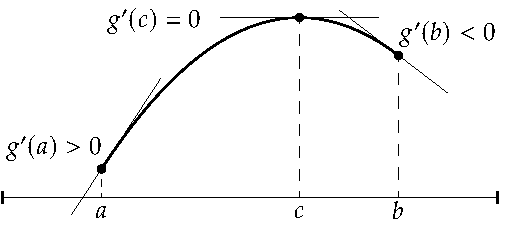
\includegraphics{../figures/darbouxthmfig}}
\end{center}

\end{frame}

\begin{frame}

\begin{theorem}[Darboux]
Let $f \colon [a,b] \to \R$ be differentiable.  Suppose $y \in \R$ is such
that $f'(a) < y < f'(b)$ or
$f'(a) > y > f'(b)$.
Then there exists a $c \in (a,b)$ such that $f'(c) = y$.
\end{theorem}

\pause
\textbf{Proof:}
Suppose 
$f'(a) < y < f'(b)$.
\pause
Define
$g(x) \coloneqq yx - f(x)$.

\pause
$g$ is continuous on $[a,b]$, and so $g$ attains a maximum at some $c \in [a,b]$.

\pause
$g$ is differentiable on $[a,b]$ and $g'(x) = y-f'(x)$
\pause
\wthus $g'(a) > 0$.

\pause
\medskip
\thus \quad $\exists$ $x > a$ such that
$\displaystyle \frac{g(x)-g(a)}{x-a} > 0$.

\pause
\medskip

\thus \quad $g(x) > g(a)$
\pause
\wthus $g$ does not have a maximum at $a$.

\pause
\medskip

Similarly, $g'(b) < 0$, so $\exists$ $x < b$ such that
$\frac{g(x)-g(b)}{x-b} < 0$ or $g(x) > g(b)$,

\pause
\thus \quad $g$ does not have a maximum at $b$.

\pause
\medskip

\thus \quad $c \in (a,b)$ and the lemma applies  \wthus $g'(c)=0$
\pause
\wthus $f'(c) = y$.

\pause
\medskip

If $f'(a) > y > f'(b)$, consider $g(x) \coloneqq f(x)- yx$.
\qed

\end{frame}

\begin{frame}
\textbf{Example:}
Define $f \colon \R \to \R$ by
\begin{equation*}
f(x) \coloneqq
\begin{cases}
{\bigl( x \sin(\nicefrac{1}{x}) \bigr)}^2 & \text{if } x \not= 0, \\
0 & \text{if } x = 0.
\end{cases}
\end{equation*}
\pause
Claim 1: $f$ is differentiable, but $f' \colon \R \to \R$ is not continuous at
$0$.

\pause
\medskip

Claim 2: $f$ has a min at $0$, but $f'$
changes sign infinitely often near $0$.

\pause
\medskip

\scalebox{0.7}{
\subimport*{../figures/}{nonc1diff_full.pdf_t}
}

\medskip

The graph of $f$ and $f'$.  The dashed line represents $f(x) \leq x^2$.

\end{frame}

\begin{frame}

$f(x) = {\bigl( x \sin(\nicefrac{1}{x}) \bigr)}^2$ if $x \not= 0$, and $f(0) = 0$.

\medskip

Claim 1: $f$ is differentiable, but $f' \colon \R \to \R$ is not continuous at
$0$.

\medskip

Claim 2: $f$ has a min at $0$, but $f'$
changes sign infinitely often near $0$.

\pause
\medskip

\textbf{Proof of claims:}
$f$ clearly has min at $0$ (as $f(x) \geq 0$ for all $x$).

\pause
\medskip

For $x \not= 0$,
$f$ is differentiable
and
$f'(x) = 2 \sin (\nicefrac{1}{x}) \bigl( x \sin (\nicefrac{1}{x}) -
\cos(\nicefrac{1}{x}) \bigr)$.

\pause
\medskip

\textbf{Exercise:} $\lim\limits_{x\to 0} f'(x)$ DNE (switches sign
infinitely often)

\pause
\medskip

For $x \neq 0$, consider

\medskip

\quad
$\displaystyle
\abs{\frac{f(x)-f(0)}{x-0} - 0}
\pause
=
\abs{\frac{x^2 \sin^2(\nicefrac{1}{x})}{x}}
\pause
=
\abs{x \sin^2(\nicefrac{1}{x})}
\pause
\leq
\abs{x}$.

\pause
\medskip

$\abs{x} \to 0$ as $x \to 0$
\pause
\wthus $f'(0)$ exists and $f'(0) = 0$. \qed

\end{frame}

\begin{frame}

\textbf{Remark:}
If $f \colon I \to \R$ is differentiable and
$f'$ is continuous on $I$, then say $f$ is
\emph{continuously differentiable}.

\pause
\medskip

One writes $C^1(I)$ for the set of continuously differentiable functions on $I$.

\end{frame}

\begin{frame}

\textbf{Exercise:}
Prove the following version of L'H\^opital's rule:

\pause
Suppose 
$f \colon (a,b) \to \R$, $g \colon (a,b) \to \R$ are differentiable
and $c \in (a,b)$.
\pause
Suppose that $f(c) = 0$, $g(c)=0$,
$g'(x) \not= 0$ when $x \not= c$, and
that the limit of $\nicefrac{f'(x)}{g'(x)}$ as $x$ goes to $c$ exists.
\pause
Show that
\begin{equation*}
\lim_{x \to c} \frac{f(x)}{g(x)} = 
\lim_{x \to c} \frac{f'(x)}{g'(x)} .
\end{equation*}
\pause
Compare to the simpler version from before.

\pause
Note: Before you do anything else, prove that $g(x) \not= 0$ when $x \not= c$.

\pause
\medskip

\textbf{Exercise:}
Prove the theorem Rolle actually proved in 1691:
\pause

\medskip

\emph{If $f$ is a polynomial,
$f'(a) = f'(b) = 0$ for some $a < b$,
and there is no $c \in (a,b)$ such that $f'(c) = 0$,
then there is at most one root of $f$ in $(a,b)$,
that is at most one $x \in (a,b)$ such that $f(x) = 0$.}
\pause

\medskip

I.e., between any two consecutive roots of $f'$ is at most one
root of $f$.

\end{frame}

\end{document}
